\documentclass{article}
\usepackage{amsmath}
\usepackage{amssymb}
\usepackage{graphicx}
\begin{document}

\section{Phase King algorithm}

The algorithm runs for $f+1$ phases, where $f$ is the number of malicious processes.
We need $f < \texttt{ceil}(n/4)$. In phase $1 \leq 1 \leq f + 1$, the process
with process id $p_i$ is the "king", which is used to break ties. 

\subsubsection{Example run with 2 faulty, 7 processes}

This algorithm cannot work in this case. We need $f < \texttt{ceil}(n/4)$, or $n > 4 f$.
However:

$$(n=7) \underset{?}{>} (4f = 4*2 = 8) = \texttt{false}$$

Assume we have this allocation of 0/1 values to
the processes, where a $M$ above a process means it is malicious.

\begin{figure}[h]
\centering
\begin{tabular}{lccccccc}
  Id         &1 & 2 & 3 & 4 & 5 & 6 & 7 \\
  Malicious? &  &   &   &   &   & M & M \\
  Value      &0 & 0 & 1 & 1 & 1 & 0 & 0 \\
\end{tabular}
\end{figure}

In this case, the actual majority is $0$ since 4 processes have value $0$,
while only $3$ have 1. However, along the non-fauly processes $[1\cdots 5]$,
we have two 0s and three 1s. Thus, the non-faulty processes can be fooled
to believe that the majority is $1$, not $0$. The non-faulty processes simplt
do not have enough information to conclude that the \textbf{actual majority} is $0$.
Hence, there is no way to actually reach consensus on $0$.

The bounds for Byzantine agreement is $f \leq \texttt{floor}(n/3)$; This is
an easier bound to fulfil, since we are
solving \textbf{agreement} \textbf{not consensus}. In the agreement problem,
everyone needs to agree on what \textbf{one person}(the general) said;
This is different from consensus, where everyone \textbf{pools together information}
together to come to a consensus.

\subsubsection{Preferred over oral message}

\textbf{Message complexity:}
For this algorithm, we only need polynomial number of messages. We have
$f+1 \simeq O(n)$ phases, and in each phase we send $O(n^2)$ messages. So in total, 
we need $O(n^3)$ messages. 

This is in contrast to the oral message algorithm where we need to
send $O(n^f)$ messages, which is not polynomial in $n$ (it is pseudopolynomial).




\section{Distributed MST: Gallager-Humblet-Spira}
\subsubsection{Complexity}

When a node is at a given level (other than 0), it can
receive at most one (a) initiate and one (b) accept. It can transmit at most one
successful (c) test message, one (d) report message, and one (e) change-root or connect
message. Since $\log_2 N$ is an upper bound on the highest level, a node can go
through $\log_2 N - 1$ levels (except 0th level), we have in total $5N (\log_2 N - 1)$ messages. 

When a node is isolated (level 0), each node can receive at most one (a) initiate
message and can transmit at most one (b) connect message, after which it will join
someone else. This will be less than $5N$ messages.

This gives a total of $5N \log_2 N$ messages.






\subsubsection{Making it work with duplicate edge weights, unique node IDs}
We can augment the edge weight information used for naming fragments
with $(\text{edge-weight}, \text{source-node-id}, \text{dest-node-id})$. As
long as the node IDs can be totally ordered, the full triple will be
totally ordered, and will give us unique names for edges. This will ensure
that we receive unique names for fragment combinations.

\subsubsection{Example}

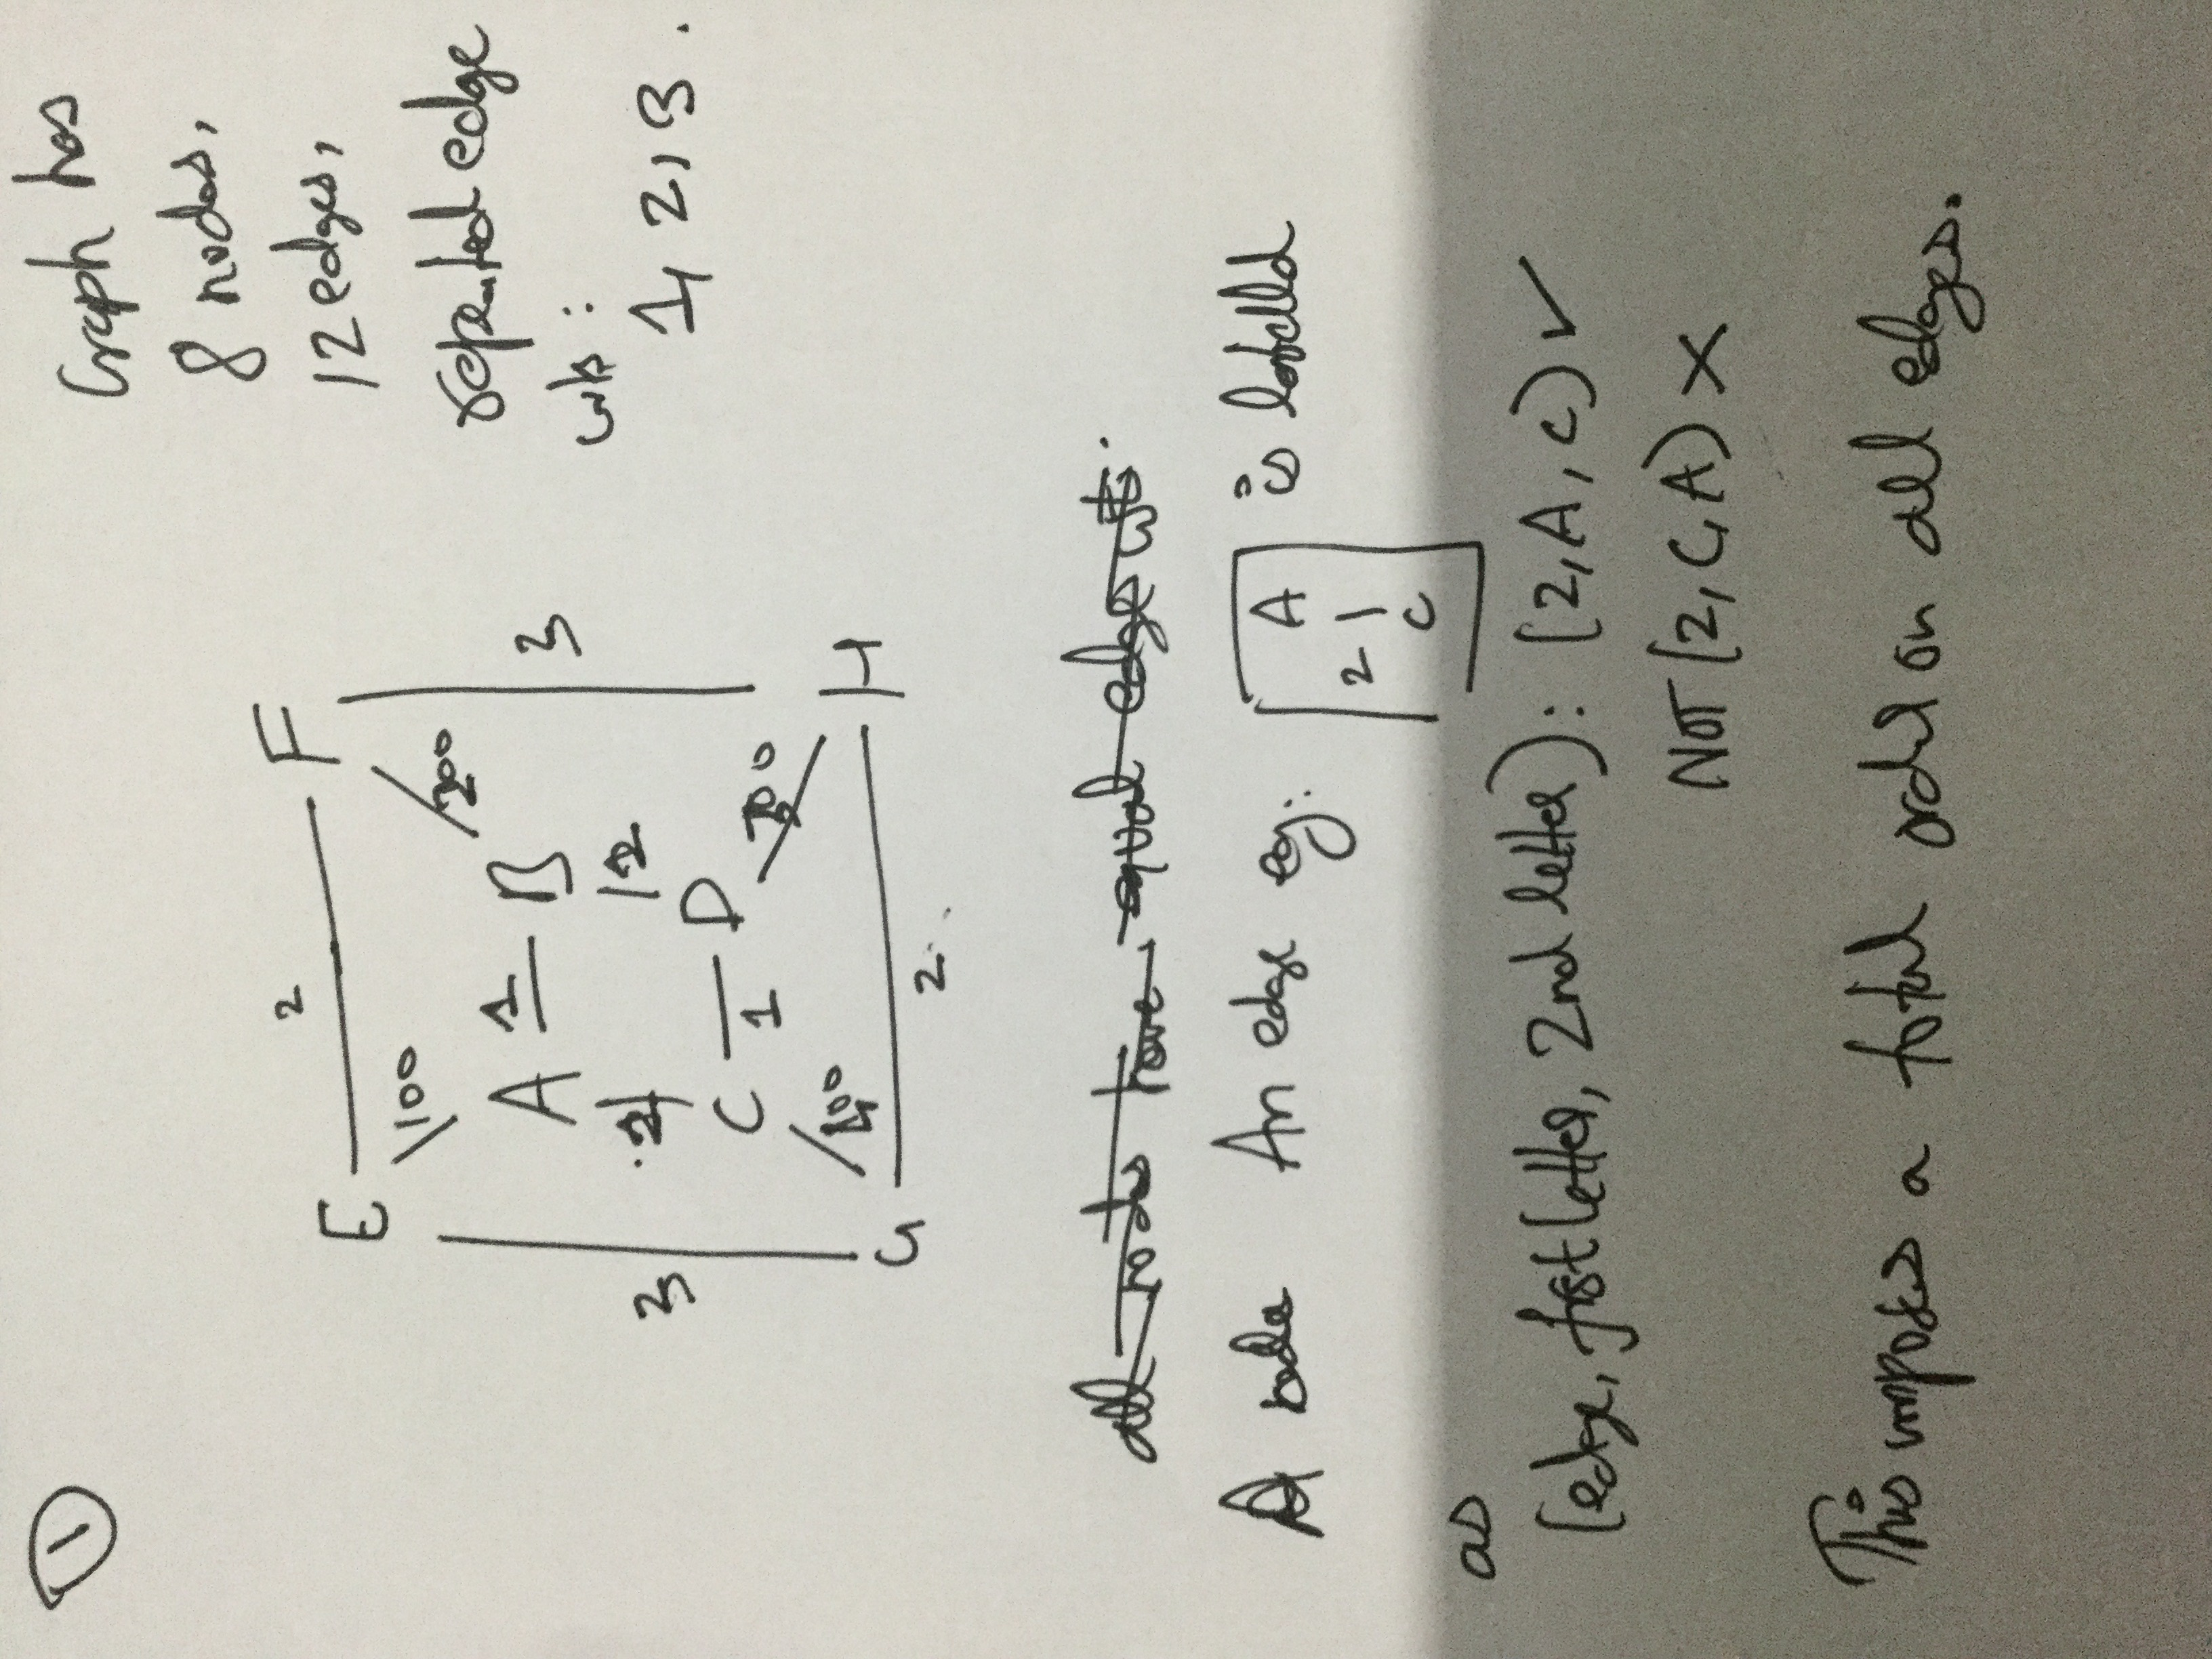
\includegraphics[width=1\textwidth, angle=270]{IMG_0626.JPG}
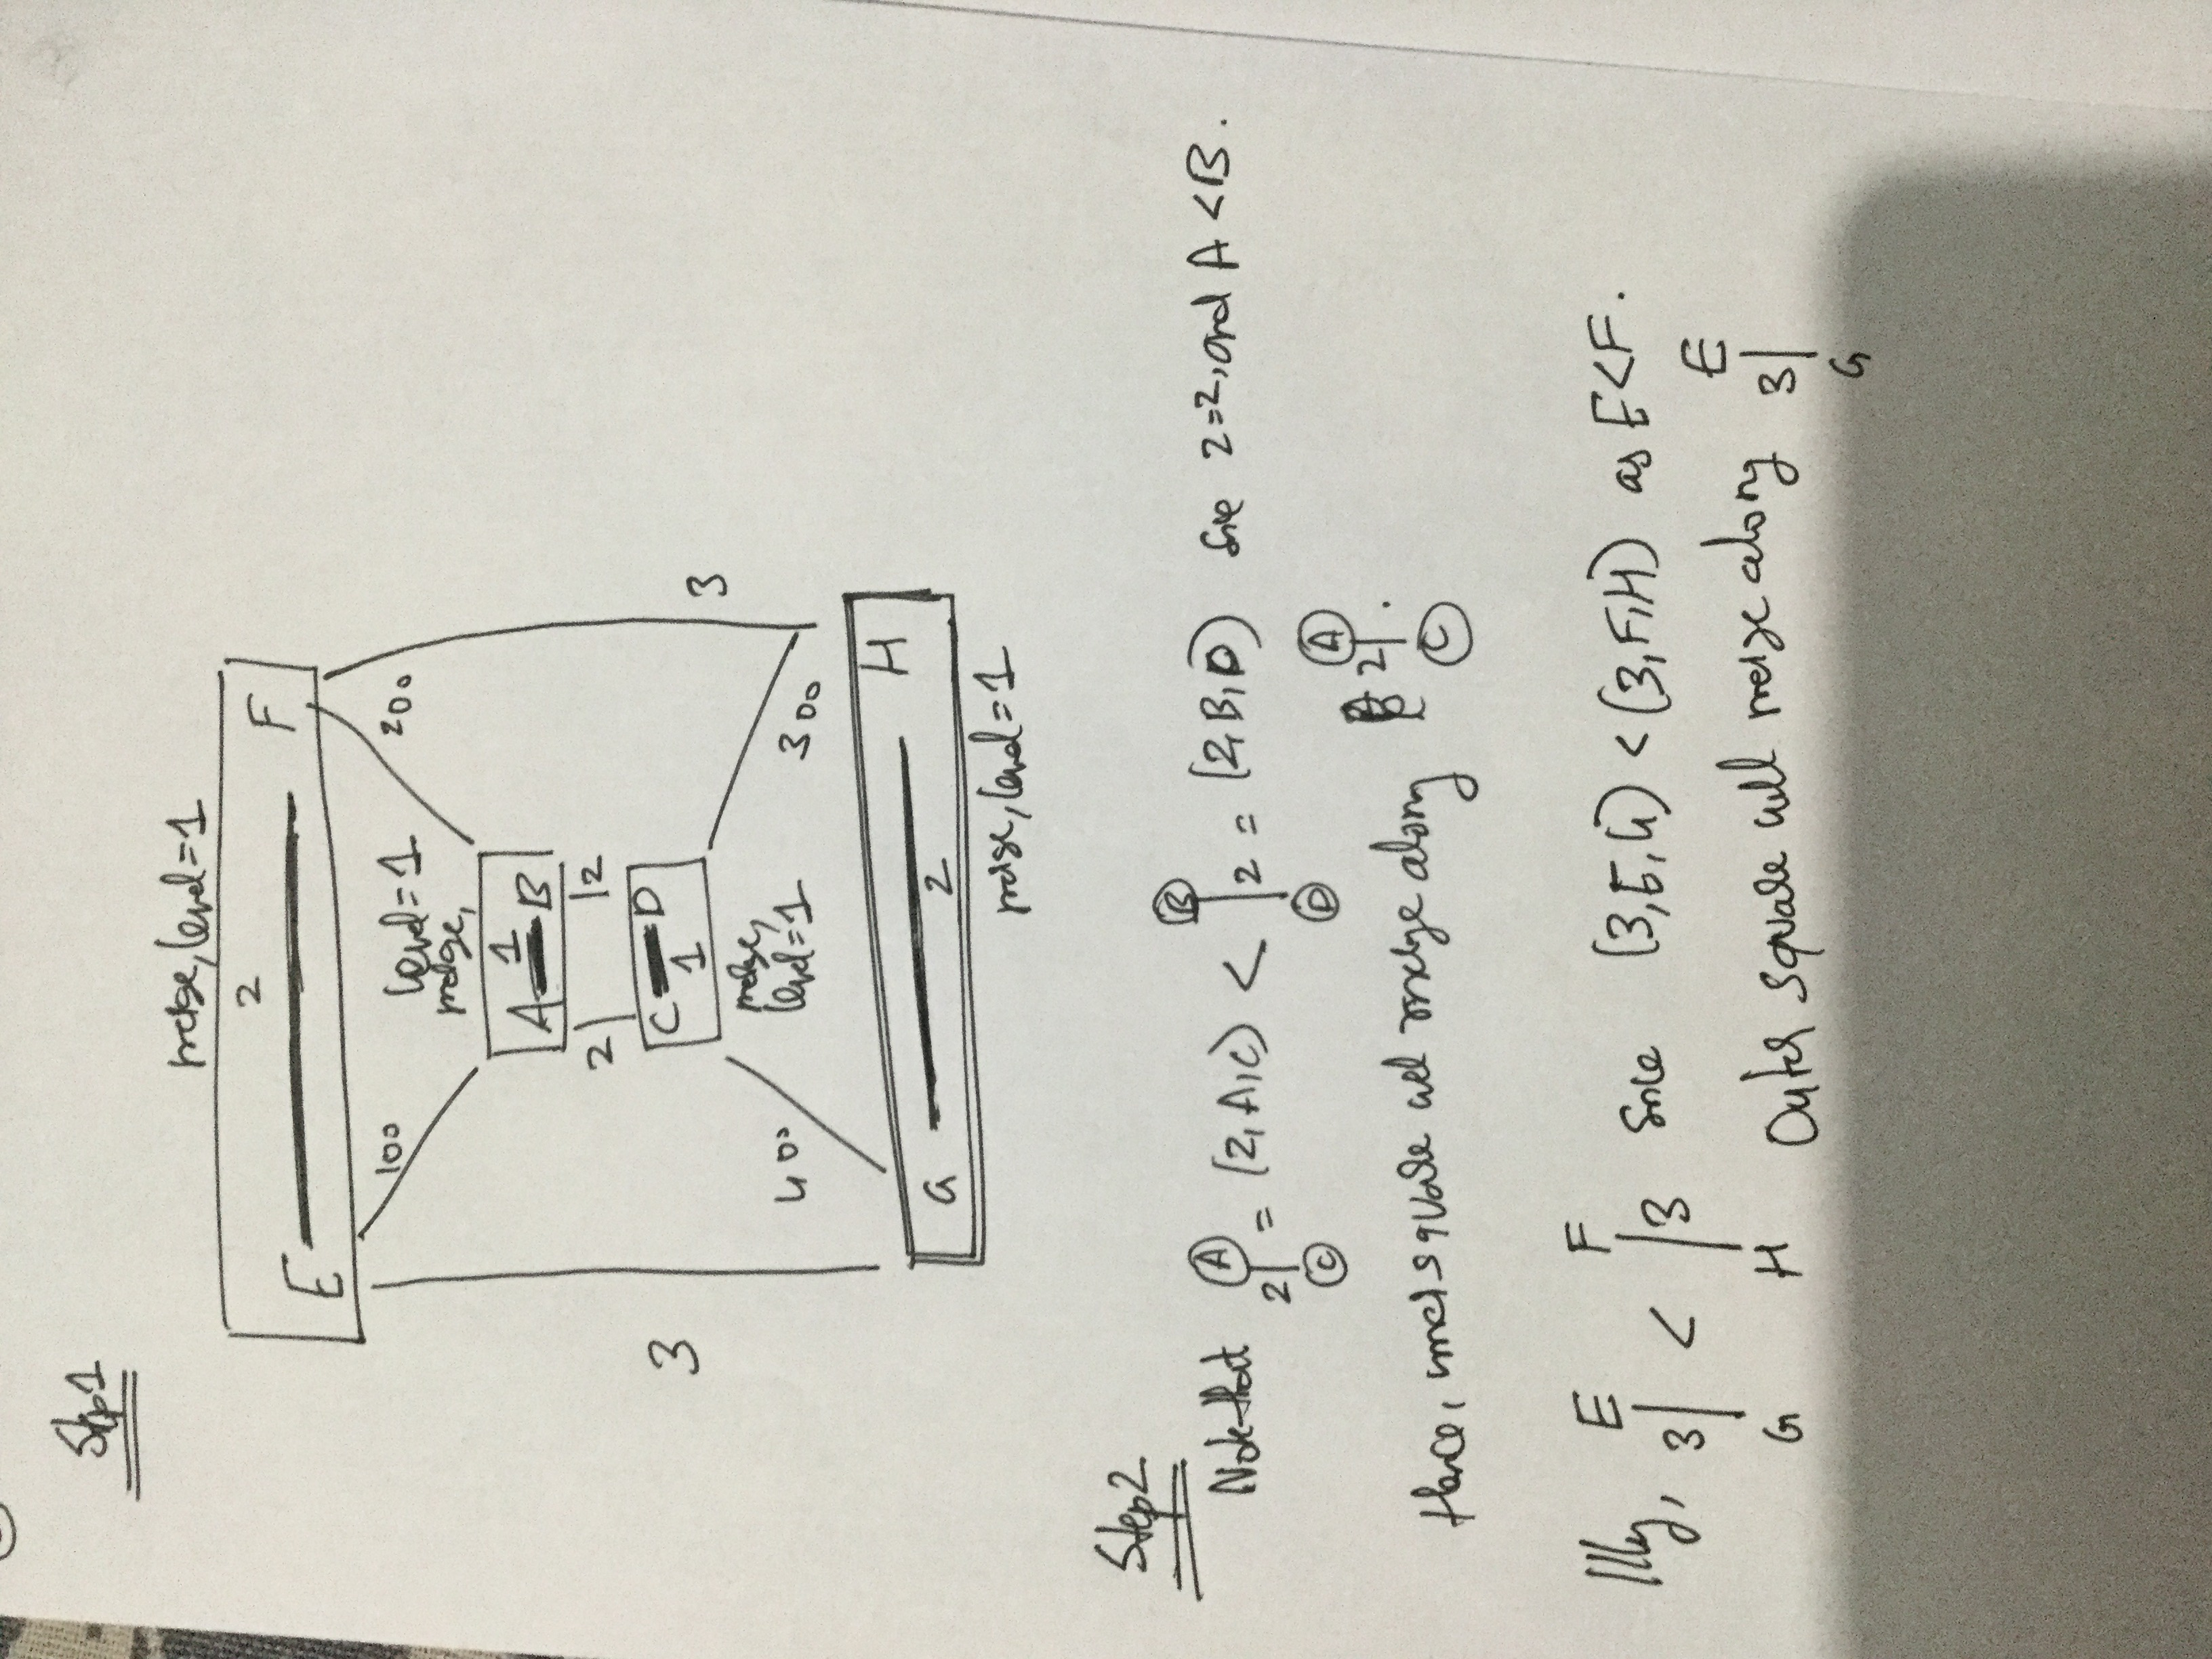
\includegraphics[width=1\textwidth, angle=270]{IMG_0627.JPG}
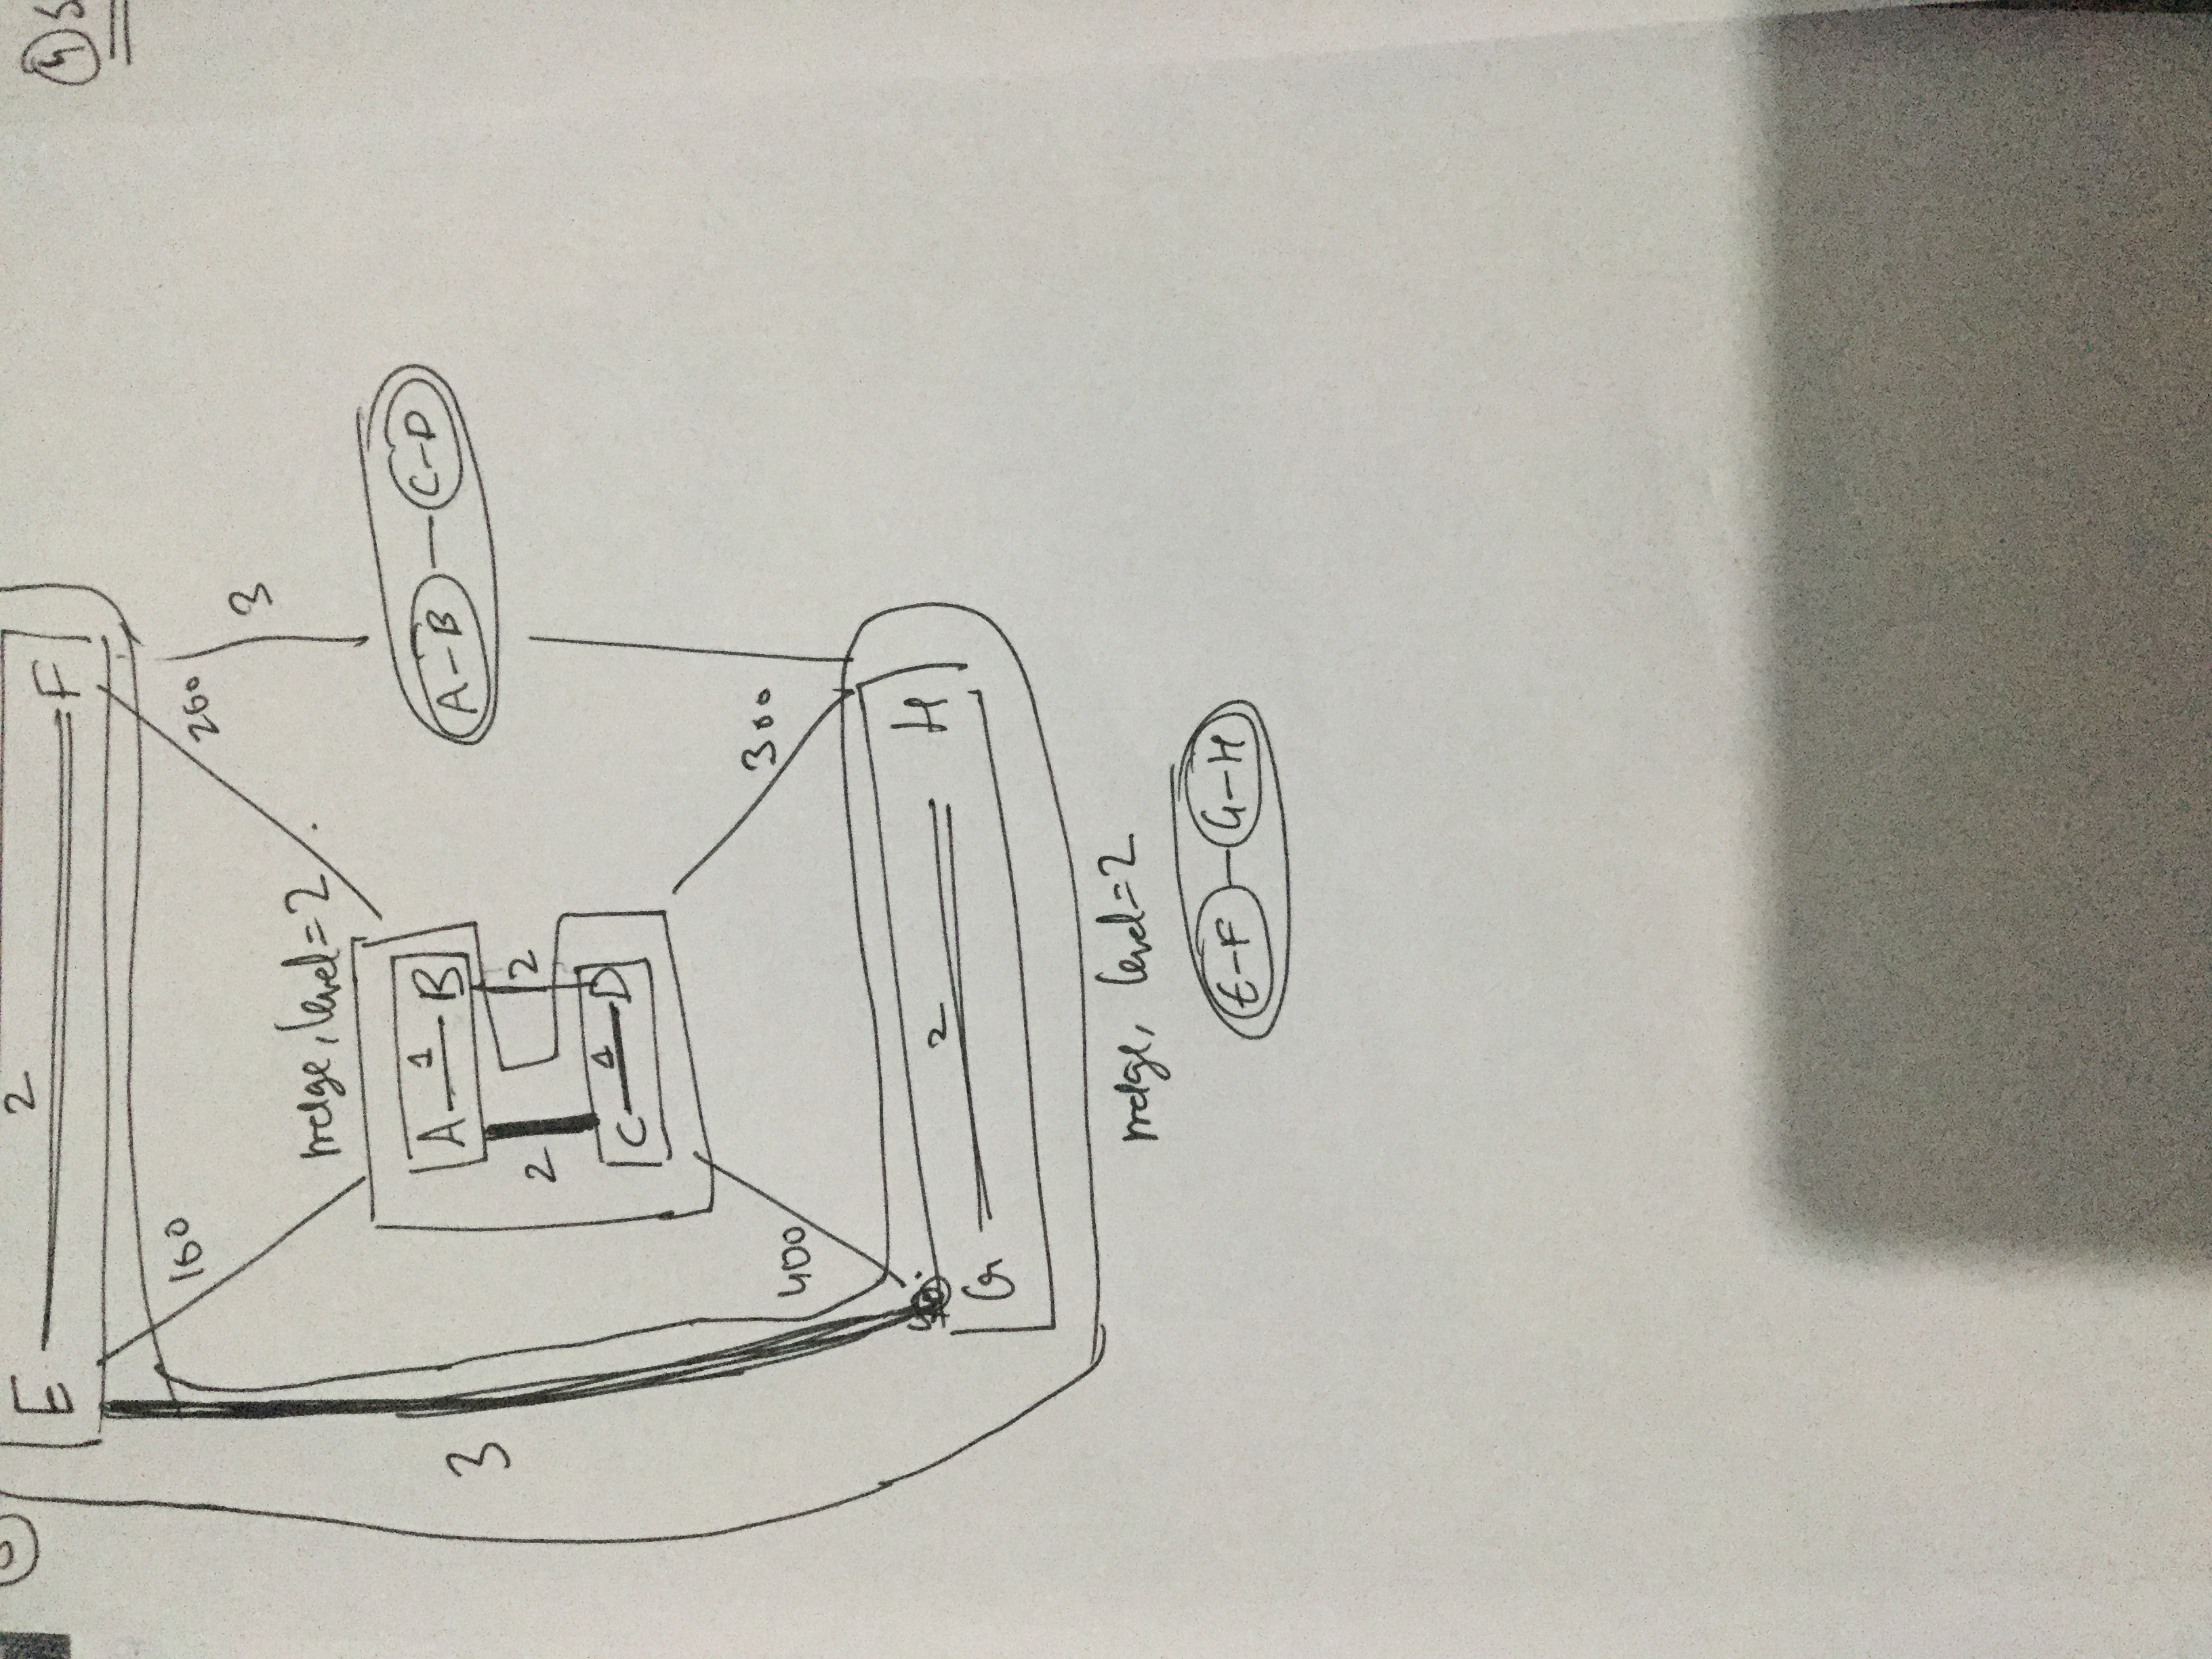
\includegraphics[width=1\textwidth, angle=270]{IMG_0628.JPG}
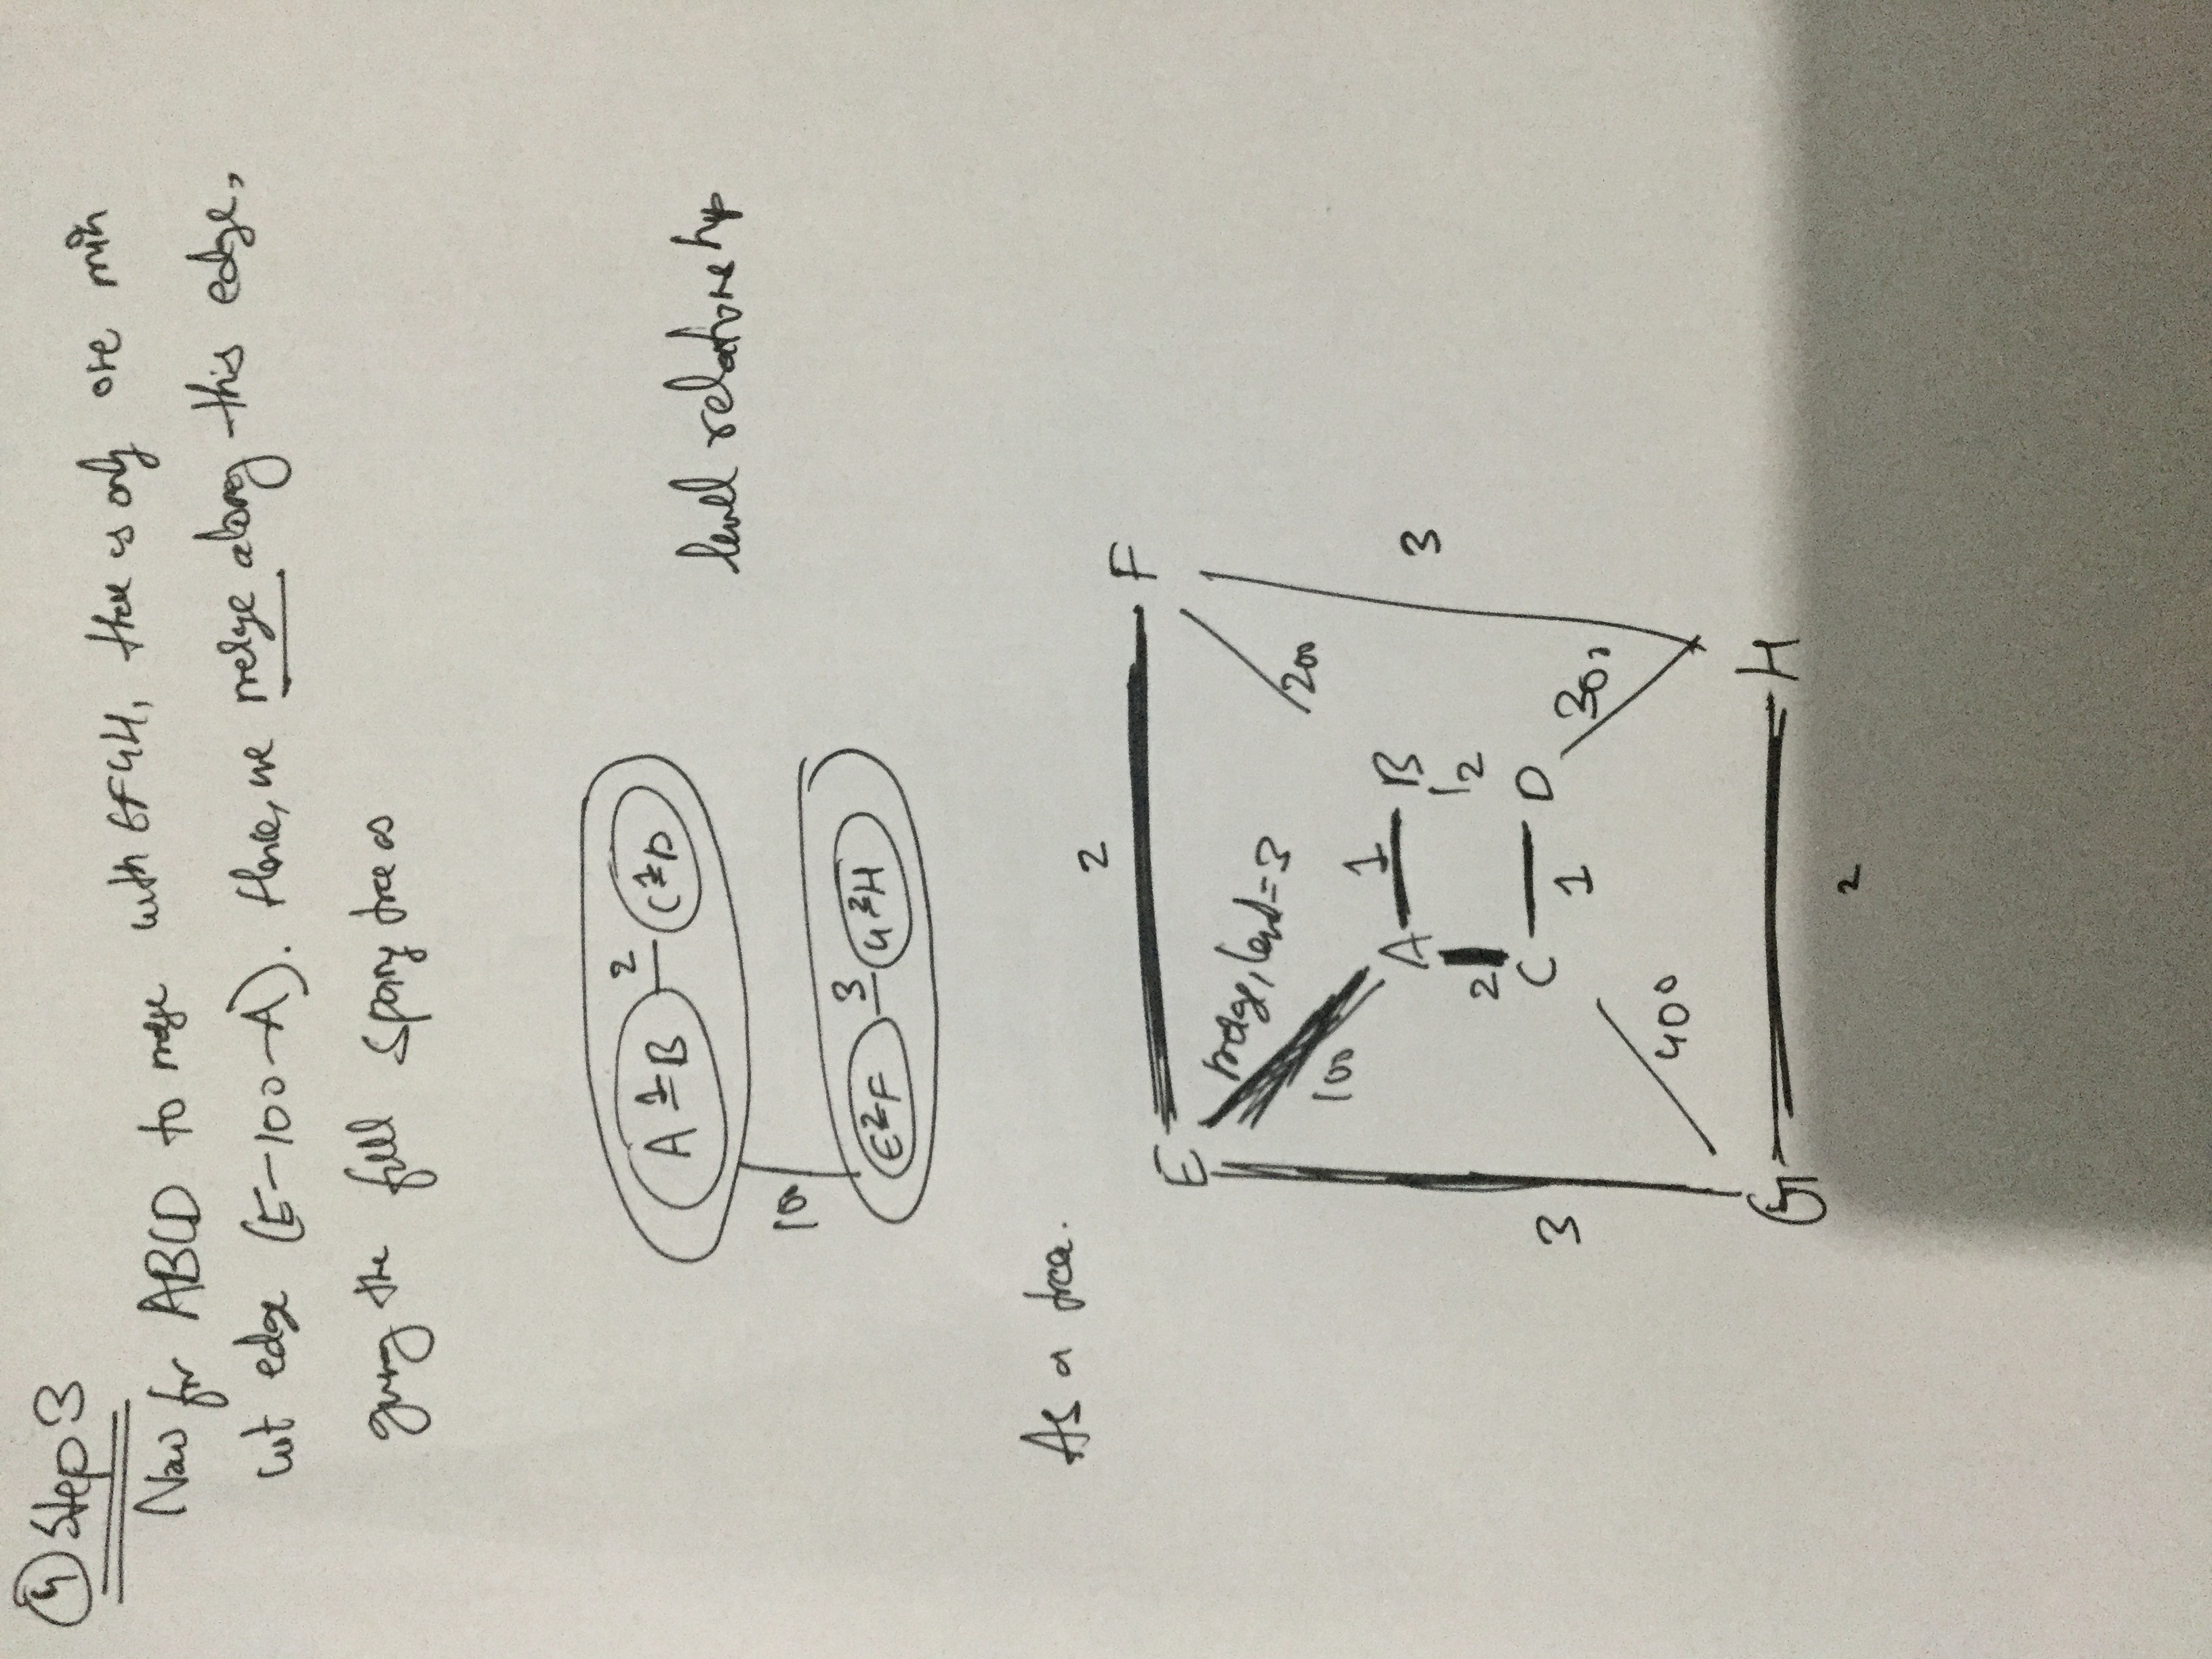
\includegraphics[width=1\textwidth, angle=270]{IMG_0629.JPG}

\subsubsection{Does the algorithm work with non-unique edge ids, node weights?}
We can make it work by slightly jittering the edge weights. For each edge $e \in E$
make a new edge $e' \in E'$ as $e' \equiv e + \epsilon_e$, where $\epsilon_e$ 
is some small, random weight that is added to the edge $e$. This ensures that
our edge weights will be distinct. 

Alternatively, we can have nodes choose random IDs. This has very small probability
of failing; Once this is done, we can then run the algorithm as explain with
"duplicate edge weights, unique node IDs".

If we do not accept small chances of error, then this is impossible.
Consider 3 nodes (which non-unique IDs) in a triangle where all edges have
weight $1$.  No node can distinguish itself from its
neighbours. Hence, if the code for one node does something, it will do the
same thing for all of them.

For any node, its outgoing edges form a minimum spanning tree. Let us say
some node $n \in \{1, 2, 3\}$ chooses to make a spanning tree. The code which is the
same on the other two nodes, and has no way of distinguishing $n$ from $n'$
will also execute the same code. Thus, the nodes cannot "agree" on a spanning
tree.

\section{True/False Question: Distributed MST}
\subsubsection{Question:}
True/False: Let $G$ be a graph and let $T$ be its MST. The minimum distance between any two nodes $u, v \in V(G)$
as measured in the minimum spanning tree $d_T(u, v)$ gives a good (non-trivial) upper
bound on the minimum distance between $u$ and $v$ in the original graph, $d_G(u, v)$.

Alternatively, is the relation $d_G(u, v) < d_T(u, v)$ useful for all choices
of $G, u, v, T$, where $T$ is guaranteed to be a minimum spanning tree of $G$.

\subsubsection{Answer:} No it does not; consider $G$ to be $N$ nodes arranged
in a ring. Label the vertices $u_0, u_2, \dots u_{N-1}$. We can
make a spanning tree $T$ for this topology by disconnecting any two nodes, say $(u_0, u_1)$.

Now, the min distance between $u_0, u_1$ in the spanning tree is $N-1$. Their
min distance in the original graph is $1$. 

Thus, in general, a spanning tree is useless for estimating distances in
the original graph. In this case, the bound gives us:

$$
1 = d_G(u_0, u_1) < d_T(u_0, u_1) = N - 1 \simeq \texttt{diameter}(G)
$$

Which is useless. We already know by the worst case that $d_G(u_0, u_1) \leq \texttt{diameter}(G)$.

\begin{figure}[h]
\centering
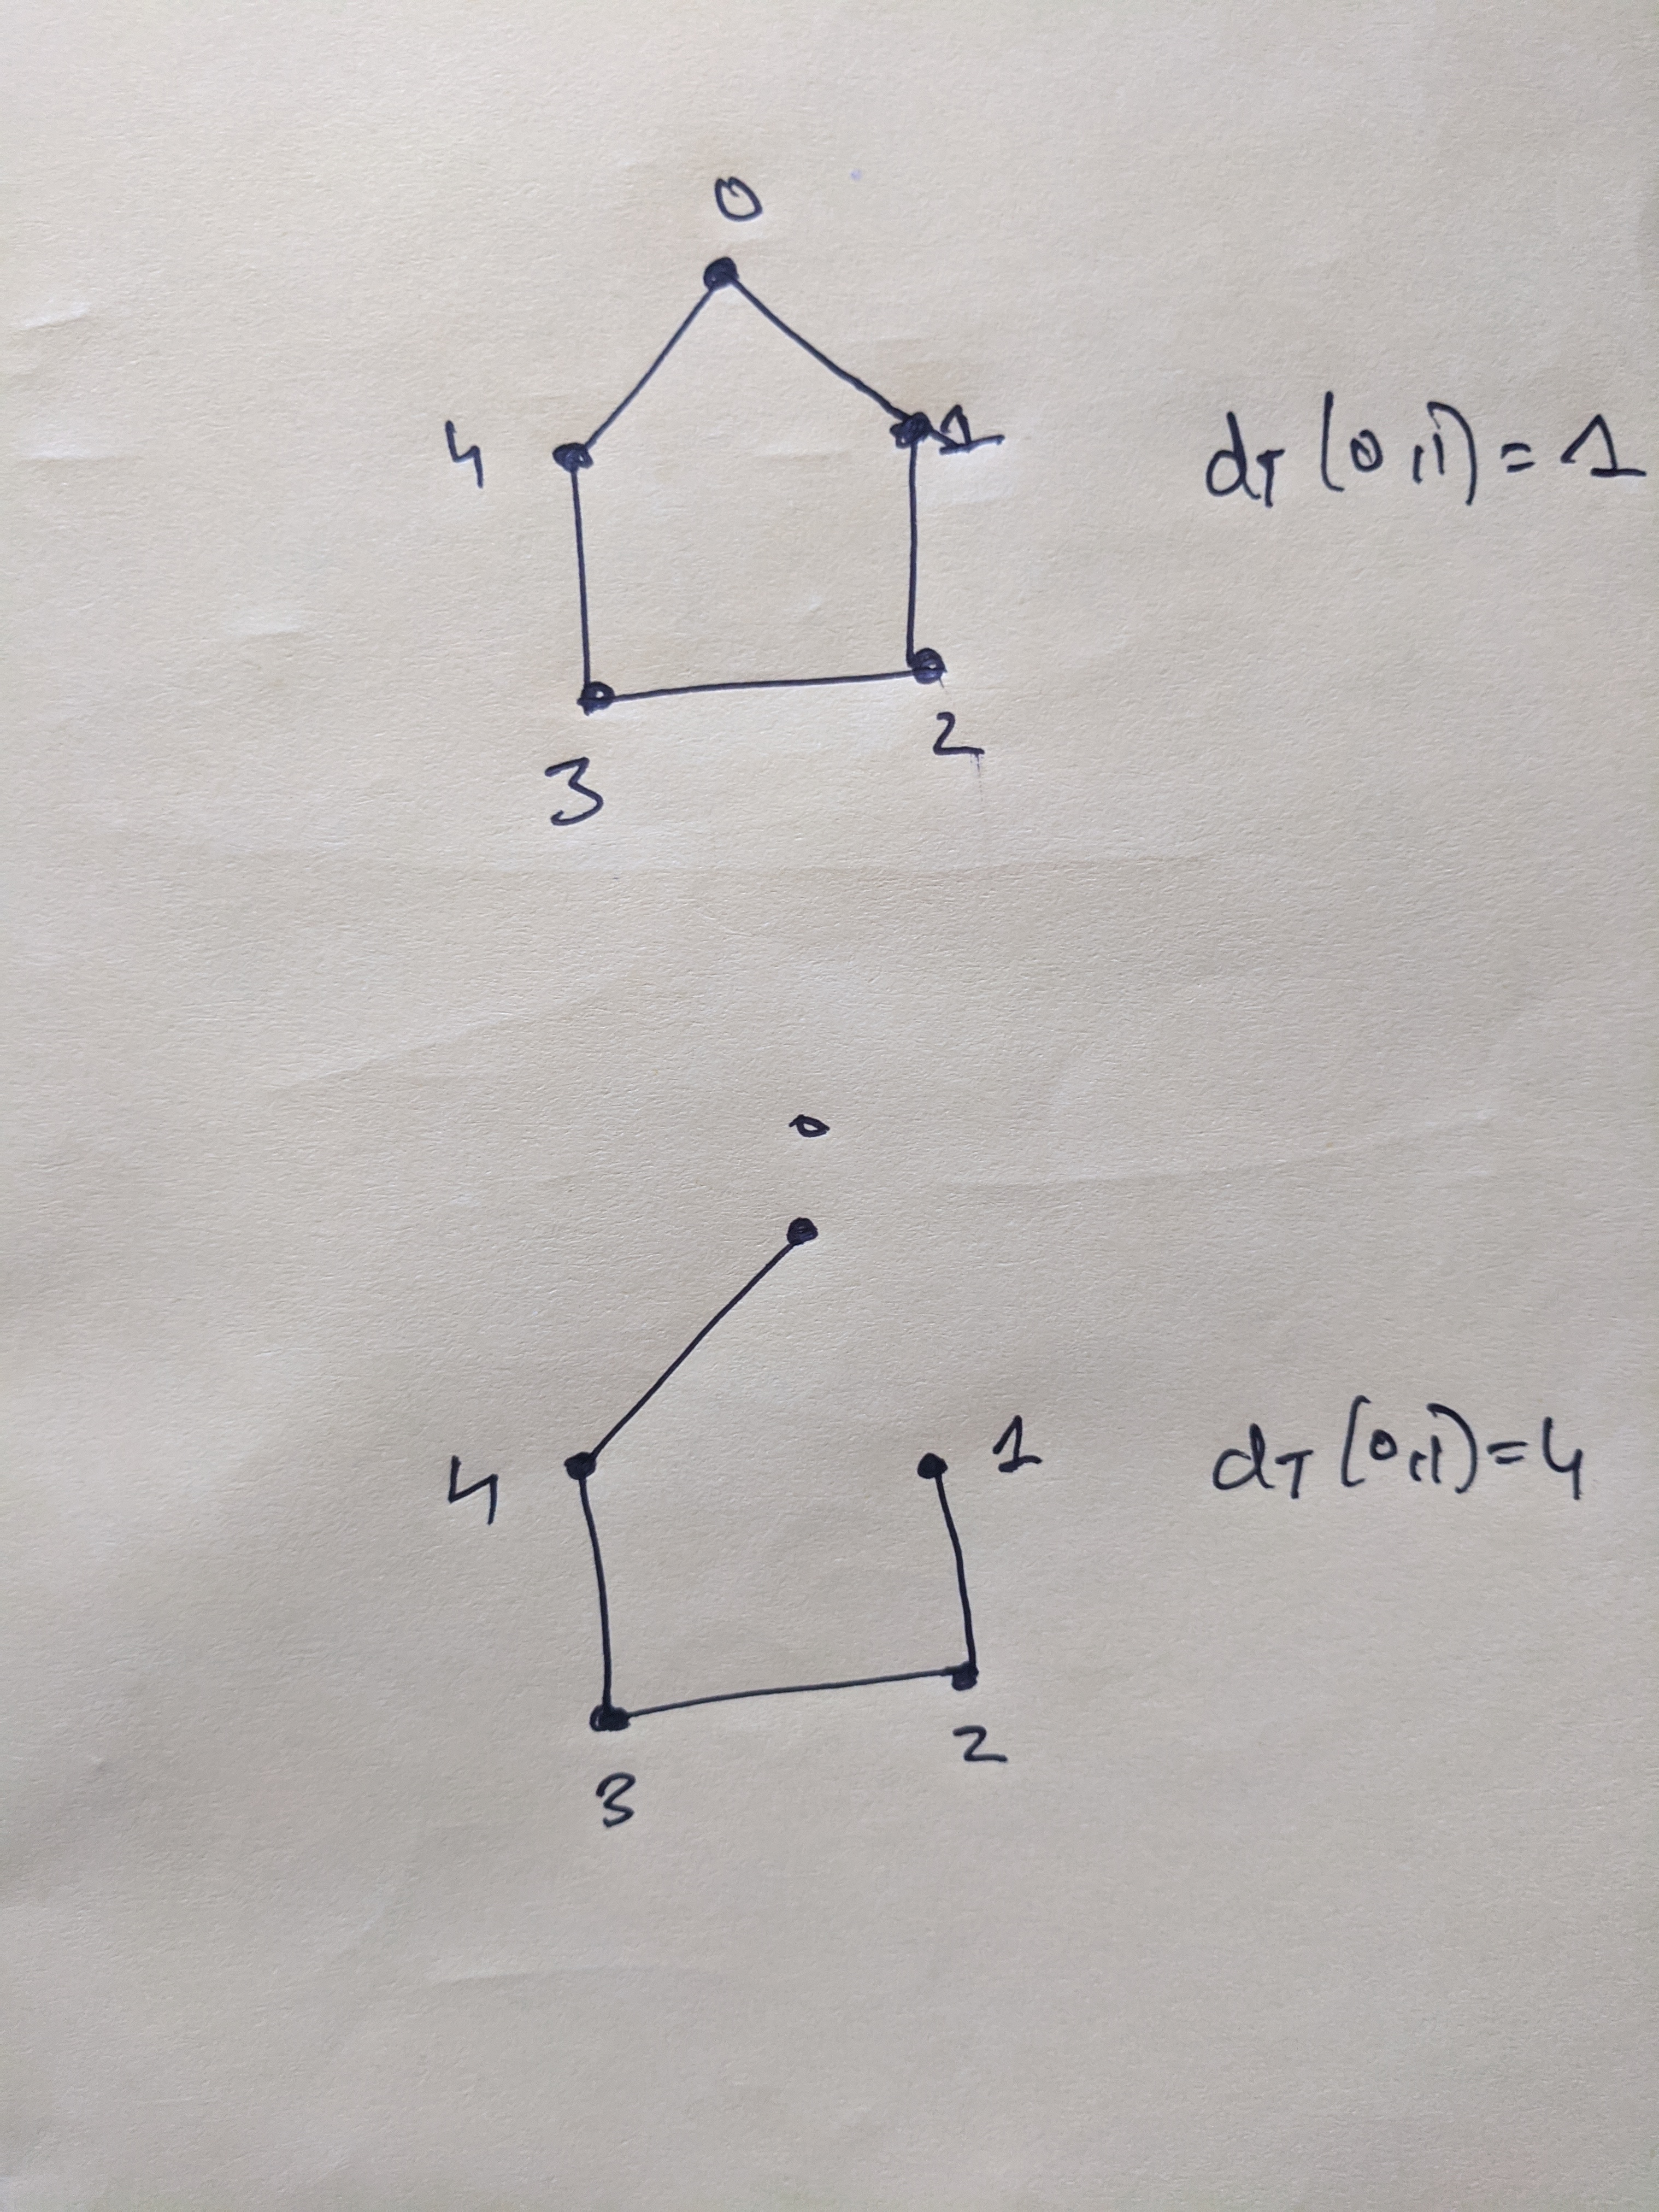
\includegraphics[width=0.5\textwidth]{graph-spanning-tree.jpg}
\caption{Example of ring with $5$ nodes; relationship b/w spanning tree distance and graph distance}
\end{figure}

\end{document}
